\documentclass[letterpaper,12pt]{article}

\usepackage{amsmath, amsfonts, amscd, amssymb, amsthm}
\usepackage{graphicx}
%\usepackage{import}
\usepackage{versions}
\usepackage{crop}
\usepackage{multicol}
\usepackage{graphicx}
\usepackage{makeidx}
\usepackage{hyperref}
\usepackage{ifthen}
\usepackage[format=hang,font=normalsize,labelfont=bf]{caption}
\usepackage{natbib}
\usepackage{setspace}
\usepackage{placeins}
\usepackage{framed}
\usepackage{enumitem}
\usepackage{threeparttable}
\usepackage{geometry}
\geometry{letterpaper,tmargin=1in,bmargin=1in,lmargin=1in,rmargin=1in}
\usepackage{multirow}
\usepackage[table]{xcolor}
\usepackage{array}
\usepackage{delarray}
\usepackage{lscape}
\usepackage{float,color, colortbl}
%\usepackage[pdftex]{graphicx}
\usepackage{hyperref}
\usepackage{tabu}
\usepackage{appendix}
\usepackage{listings}


\include{thmstyle}
\bibliographystyle{aer}
\providecommand{\abs}[1]{\lvert#1\rvert}
\providecommand{\norm}[1]{\lVert#1\rVert}
\newcommand{\ve}{\varepsilon}
\newcommand{\ip}[2]{\langle #1,#2 \rangle}

\hypersetup{colorlinks,linkcolor=red,urlcolor=blue,citecolor=red}
\theoremstyle{definition}
\newtheorem{theorem}{Theorem}
\newtheorem{acknowledgement}[theorem]{Acknowledgement}
\newtheorem{algorithm}[theorem]{Algorithm}
\newtheorem{axiom}[theorem]{Axiom}
\newtheorem{case}[theorem]{Case}
\newtheorem{claim}[theorem]{Claim}
\newtheorem{conclusion}[theorem]{Conclusion}
\newtheorem{condition}[theorem]{Condition}
\newtheorem{conjecture}[theorem]{Conjecture}
\newtheorem{corollary}[theorem]{Corollary}
\newtheorem{criterion}[theorem]{Criterion}
\newtheorem{definition}{Definition} % Number definitions on their own
\newtheorem{derivation}{Derivation} % Number derivations on their own
\newtheorem{example}[theorem]{Example}
\newtheorem{exercise}[theorem]{Exercise}
\newtheorem{lemma}[theorem]{Lemma}
\newtheorem{notation}[theorem]{Notation}
\newtheorem{problem}[theorem]{Problem}
\newtheorem{proposition}{Proposition} % Number propositions on their own
\newtheorem{remark}[theorem]{Remark}
\newtheorem{solution}[theorem]{Solution}
\newtheorem{summary}[theorem]{Summary}
%\numberwithin{equation}{document}
\graphicspath{{./Figures/}}
\renewcommand\theenumi{\roman{enumi}}
\DeclareMathOperator*{\argmin}{arg\,min}

\crop
\makeindex


\begin{document}

\begin{titlepage}
	\title{Open Source Macroeconomics Laboratory Boot Camp \\ Perturbation Methods}  %change title here accordingly
	\author{Kerk Phillips\\ \emph{Congressional Budget Office}}
	\date{\LARGE{2019}}
	\maketitle
\end{titlepage}

\begin{spacing}{1.5}

\section{Introduction} \label{Perturb_Intro}
	In this section we will explore in more detail the perturbation methods referenced in section 5.4 of the DSGE chapter. We will only consider a second order approximation of the policy function here, but approximations of yet higher order follow the same basic approach. There are many alterations of the standard perturbation method. Detailed discussions of perturbation methods can be found in chapters  13 -- 15 of \citet{Judd1998}, as well as in \citet{CollardJuilliard2001}, \citet{SchmittGroheUribe2004}, and \citet{HeerMaussner2009}.

	As noted previously, assuming that the policy functions are linear can be extremely useful in solving DSGE models. When second or higher order properties of the characterizing equations of the are important to the question being answered, however, linearization is undesirable. Linearization is essentially a first order Taylor series approximation about the steady state, as discussed in section 6 of the DSGE chapter. Such an approximation results in certainty equivalence, or the phenomenon of unconditional expectations of the endogenous variables being equal to their non-stochastic steady state values. This occurs because in a linear approximation, only the first moments of the shocks enter the linear equations. As these processes are assumed to be mean zero, these moments wash out when expectations are taken. Thus, the distribution of the shocks have no influence on the resultant policy equation solutions. 

	Applications where this can be troublesome include asset pricing models and welfare analysis. In asset pricing models the riskiness of an asset is directly related to the variance of the underlying shocks. Thus, failing to account for higher order characteristics of the model can invalidate the results. In welfare analysis where the utility functions have high curvature, failing to account for the second moment can similarly produce spurious results.

\section{Pertubation Methods in General} \label{Perturb_General}
	To see how perturbation methods work consider the following simple example.  Suppose we have a condition on a potentially nonlinear bivariate function:
	\begin{equation} \label{Perturb_Fxu}
	 F(x,u) = 0
	\end{equation}
	Assume $u$ is an exogenously given variable, and $x$ will be choson to satisfy \eqref{Perturb_Fxu}.   Denote the solution to this condition as $x(u)$ and assume that the value of $x(u_0)$ is known.

	Taking the derivative of \eqref{Perturb_Fxu} with respect to $u$ gives:
	\begin{equation} \label{Perturb_Fxu1derv}
	 F_x\{x(u),u\} x_u(u) + F_u\{x(u),u\}= 0
	\end{equation}
	If we evaluate this at $u=u_0$ and solve for the first derivative of $x(u)$, we have:
	\begin{equation} \label{Perturb_linear}
	x_u(u_0) = -\frac{F_u\{x(u_0),u_0\}}{F_x\{x(u_0),u_0\}}
	\end{equation}
	Since $x(u_0)$ is known, as long as $F_x\{x(u_0),u_0\} \ne 0$ we can find the value for the first derivative.
	The first-order (linear) Taylor-series approximation of $x(u)$ will be:
	\begin{equation} \label{Perturb_Taylor1}
	x(u) = x(u_0) + x_u(u_0)(u-u_0)
	\end{equation}

	To find the second-order terms we differentiate \eqref{Perturb_Fxu1derv} again with respect to $u$.
	\begin{equation} \label{Perturb_Fxu2derv}
	\begin{split}
	 & F_{xx}\{x(u),u\} x_u(u) x_u(u) + F_{xu}\{x(u),u\}x_u(u) \\
	 + & F_{x}\{x(u),u\} x_{uu}(u) + F_{xu}\{x(u),u\} x_u(u) \\
	 + & F_{uu}\{x(u),u\} =0
	\end{split}
	\end{equation}
	Again evaluating at $u=u_0$ and solving this time for the second derivative of $x(u)$, we have:
	\begin{equation} \label{Perturb_quad}
	x_{uu}(u_0) = -\frac{F_{xx}\{x(u_0),u_0\}[x_u(u_o)]^2 + 2F_{xu}\{x(u_0),u_0\}x_u(u_o) + F_{uu}}{F_x\{x(u_0),u_0\}}
	\end{equation}
	Hence, the second-order (quadratic) Taylor-series approximation of $x(u)$ will be:
	\begin{equation} \label{Perturb_Taylor2}
	x(u) = x(u_0) + x_u(u_0)(u-u_0) + \tfrac{1}{2} x_{uu}(u_0)(u-u_0)^2
	\end{equation}

	Higher order terms can be obtained by successive differentiation of \eqref{Perturb_Fxu2derv}, setting $u=u_0$ and solving for the appropriate derivative.  This will be a function of the various derivatives of $F(x,u)$ and the lower-order derivatives of $x(u)$ obtained from previous iterations.

\section{Application to a Simple DGE Model} \label{Perturb_DGE}
	Consider a simple dynamic general equilibrium model with no stochastic shocks.  An example of this is the model from \citet{BrockMirman1972}, which we have examined before.  This model can be written in the following form.
	\begin{equation}\label{Perturb_BMEuler}
		\frac{1}{K_t^\alpha - K_{t+1}} = \beta E_t \left\{\frac{\alpha K_{t+1}^{\alpha-1}}{K_{t+1}^\alpha - K_{t+2}} \right\} \nonumber
	\end{equation}

	We will rewrite this as follows.
	\begin{equation}\label{Perturb_BMEuler2}
		\frac{1}{K_t^\alpha - K_{t+1}} - \beta \frac{\alpha K_{t+1}^{\alpha-1}}{K_{t+1}^\alpha - K_{t+2}} = 0
	\end{equation}	

	We know the steady state is defined by $K_{t+2} = K_{t+1} = K_t = \bar K$.  Substituting this into \eqref{Perturb_BMEuler2} gives:
	\begin{align}
		\beta \alpha {\bar K}^{\alpha-1} = 1 \nonumber \\
		\bar K = (\beta \alpha)^{\frac{1}{1-\alpha}} \label{Perturb_BMSS}
	\end{align}	

	In terms of our notatation from the previous section we have:
	\begin{align}
		u & = K_t \nonumber \\
		x & = x(u) = K_{t+1} \nonumber \\
		y & = x(x) = K_{t+2} \nonumber \\
		F(y,x,u) & = F(y(x(u)),x(u),u) = \frac{1}{K_t^\alpha - K_{t+1}} - \beta \frac{\alpha K_{t+1}^{\alpha-1}}{K_{t+1}^\alpha - K_{t+2}} = 0 \label{Perturb_BMFeqn}
	\end{align}
	Take the derivative of \eqref{Perturb_BMFeqn} with respect to $u = K_t$:
	\begin{equation} \begin{split}
		& F_y(y(x(u)),x(u),\bar u) x_u(x(u)) x_u(u)  \\
		& + F_x(y(x(u)),x(u),u) x_u(u) + F_u(y(x(u)),x(u),u) = 0 \label{Perturb_BMFueqn}
	\end{split} \end{equation}

	Evaluating \eqref{Perturb_BMFueqn} at $u = \bar u = \bar K$ and noting that $x(\bar u) = \bar u$:
	\begin{align}
		& F_y(y(x(\bar u)),x(\bar u),\bar u) x_u(x(\bar u)) x_u(\bar u) \nonumber \\
		& + F_x(y(x(\bar u)),x(\bar u),\bar u) x_u(\bar u) + F_u(y(x(\bar u)),x(\bar u),\bar u) = 0 \nonumber \\
		& F_y(\bar u,\bar u,\bar u)\; x_u(\bar u)^2 + F_x(\bar u,\bar u,\bar u)\; x_u(\bar u) + F_u(\bar u,\bar u,\bar u)  = 0 \nonumber
	\end{align}
	Note that $F_y(\bar u,\bar u,\bar u)$ is the same as $F$ from the linearization notes.  Similarly, $F_x(\bar u,\bar u,\bar u)$ is $G$, and $F_u(\bar u,\bar u,\bar u)$ is $H$.  Also note that $x_u(\bar u)$ is $P$.  As in those notes the value of $x_u(\bar u)$ comes from a solving a quadratic.

	Now we take the derivative of \eqref{Perturb_BMFueqn} with respect to $u$ and evalauate it at $u=\bar u$.
	\begin{equation} \begin{split}
		& F_{yy}(\bar u,\bar u,\bar u)\; x_u(\bar u)^4 \\
		& + F_{yx}(\bar u,\bar u,\bar u)\; x_u(\bar u)^3 \\
		& + F_{yu}(\bar u,\bar u,\bar u)\; x_u(\bar u)^2 \\
		& + F_y(\bar u,\bar u,\bar u)\; x_{uu}(\bar u)\; x_u(\bar u)^2 \\
		& + F_y(\bar u,\bar u,\bar u)\; x_u(\bar u)\; x_{uu}(\bar u) \\
		& + F_{yx}(\bar u,\bar u,\bar u)\; x_u(\bar u)^3 \\
		& + F_{xx}(\bar u,\bar u,\bar u)\; x_u(\bar u)^2 \\
		& + F_{xu}(\bar u,\bar u,\bar u)\; x_u(\bar u) \\
		& + F_x(\bar u,\bar u,\bar u)\; x_{uu}(\bar u) \\
		& + F_{yu}(\bar u,\bar u,\bar u)\; x_u(\bar u)^2 \\
		& + F_{xu}(\bar u,\bar u,\bar u)\; x_u(\bar u) \\
		& + F_{uu}(\bar u,\bar u,\bar u) = 0 \label{Perturb_BMFuueqn}
	\end{split} \end{equation}
	Supressing the function arguments for the sake of clarity we can rewrite \eqref{Perturb_BMFuueqn} as below.
	\begin{equation} \begin{split}
		& (F_{yy}\; x_u^4 + 2F_{yx}\; x_u^3 + 2F_{yu}\; x_u^2 + F_{xx}\; x_u^2 + 2F_{xu}\; x_u + F_{uu}) \\
		& + (F_y\; x_u^2 + F_y\; x_u + F_x) x_{uu} = 0 \nonumber
	\end{split} \end{equation}
	Note the $F_{ij}$ are all second-derivatives evaluated at the steady state. Since $x_u$ has already been solved we can solve this for $x_{uu}$.  
	\begin{equation}
		x_{uu} = - \frac{F_{yy}\; x_u^4 + 2F_{yx}\; x_u^3 + 2F_{yu}\; x_u^2 + F_{xx}\; x_u^2 + 2F_{xu}\; x_u + F_{uu})}{(F_y\; x_u^2 + F_y\; x_u + F_x)} \label{Perturb_BMxuueqn}
	\end{equation}

	The quadratic approximation to the policy function is given by:
	\begin{equation}
		\tilde K_{t+1} = x_u \tilde K_t + \frac{1}{2} x_{uu} {\tilde K}_t^2
	\end{equation}

\section{Pertubation Methods in Dynamic Stochastic Equilibrium Models} \label{Perturb_Dynamic}
	In this section we will explore in more detail the perturbation methods referenced in section 5.4 of the DSGE chapter. We will only consider a second order approximation of the policy function here, but approximations of yet higher order follow the same basic approach. There are many alterations of the standard perturbation method. Detailed discussions of perturbation methods can be found in chapters  13 -- 15 of \citet{Judd:1998}, as well as in \citet{CollardJuilliard2001}, \citet{SchmittGroheUribe2004}, \citet{HeerMaussner:2009} and \citet{GommeKlein:2011}.  \citet{Binning:2012} uses similar techniques to get cubic approximations.

	Consider a non-linear system of dynamic equations.  We can take natural logs or otherwise transform the equations to get:
	\begin{equation} \label{Perturb_Gamfunc}
	E_t\{\Gamma (X_{t+1},X_t,X_{t-1},Y_{t+1},Y_t,Z_{t+1},Z_t)\} = 0
	\end{equation}
	$X$ is a set of endogenous state variables, $Y$ is a set of "jump", costate, or control variables, and $Z$ is a list of exogenous state variables.  The methods for obtaining a linear approximation of the policy function are well known from \citet{Uhlig1999}.  Our task in this section is to obtain the quadratic terms from a second-order approximation of the same policy function.

	We must recall that the exogenous state variables evolve according to a linear law of motion given in \eqref{Perturb_Zlom} with the long run value of $\bar Z = 0$.
	\begin{equation} \label{Perturb_Zlom}
	Z_t = N Z_{t-1} + v \Omega \ve_t; \ve_t \sim (0,I_{n_Z}) 
	\end{equation}
	where $v$ is a scalar, and $\Omega$ is a matrix that determines correlations of the elements in $\ve_t$.

	We are searching for the quadratic terms in the Taylor-series approximation of the policy function and jump variable functions which we will denote:
	\begin{align}
		X_{t} & = H(X_{t-1},Z_t,v) \label{Perturb_Hfunc} \\
		Y_{t} & = G(X_{t-1},Z_t,v) \label{Perturb_Gfunc}
	\end{align}

	For notational ease define the following.
	\begin{align}
		A_t & \equiv \begin{bmatrix} X_{t+1} & X_t & X_{t-1} & Y_{t+1} & Y_t & Z_{t+1} & Z_t \end{bmatrix}^T \label{Perturb_Adef} \\
		S_t & \equiv \begin{bmatrix} X_{t-1} & Z_t & v\end{bmatrix} \label{Perturb_Sdef} \\
		n_A & \equiv 3n_X + 2n_Y + 2n_Z \\
		n_s & \equiv n_X + n_Z + 1
	\end{align}

	\subsection{Definitions and Preliminaries}
		The Taylor-series approximation of $\Gamma$ with second-order terms for the variance is:
		\begin{equation} \label{Perturb_quadtermsGam}
		\begin{split}
		& \Gamma(A_t) \;\dot =\; \Gamma(\bar X, ..., \bar Z) + \begin{bmatrix} \Gamma_1 & \dots & \Gamma_7 \end{bmatrix} \begin{bmatrix} \tilde X_{t+1} \\ \vdots \\ \tilde Z_t \end{bmatrix}  \\
		+ & \frac{1}{2} \left( I_{n_A} \otimes \begin{bmatrix} \tilde X_{t+1} & \vdots & \tilde Z_t \end{bmatrix} \right) \begin{bmatrix} \Gamma_{11} & \dots & \Gamma_{17} \\  \vdots & \ddots & \vdots \\ \Gamma_{71} & \dots & \Gamma_{77} \end{bmatrix} \begin{bmatrix} \tilde X_{t+1} \\ \vdots \\ \tilde Z_t \end{bmatrix}
		\end{split}
		\end{equation}

		The Taylor-series approximation of $H$ with second-order terms for the variance is:
		\begin{equation} \label{Perturb_quadtermsH}
		\begin{split}
		& H(X_{t-1},Z_t,v) \;\dot =\; H(\bar X,\bar Z,\bar v) + \begin{bmatrix} H_X & H_Z & H_v \end{bmatrix}\begin{bmatrix} \tilde X_{t-1} \\ \tilde Z_t  \\ \tilde v \end{bmatrix} \\
		+ & \frac{1}{2} \left( I_{n_Y+n_X} \otimes \begin{bmatrix}\tilde X_{t-1}^T & \tilde Z_t^T & \tilde v \end{bmatrix} \right) \begin{bmatrix} H_{XX} & H_{XZ} & 0 \\  H_{ZX} & H_{ZZ} & 0 \\ 0 & 0 & H_{vv} \end{bmatrix} \begin{bmatrix} \tilde X_{t-1} \\ \tilde Z_t \\ \tilde v \end{bmatrix}
		\end{split}
		\end{equation}
		
		$H_X$ and $H_Z$ terms are the $P$ and $Q$ matrices in Uhlig's notation.  $H_{XX}$, $H_{ZZ}$, $H_{ZX}$, $H_{XZ}^T$ and $H_{vv}$ are all \citet{MagnusNeudecker:1999} matrices of second-order coefficients.  A similar setup is used for the approximation of the $G$ function.

		\begin{equation} \label{Perturb_quadtermsG}
		\begin{split}
		& G^k(X_{t-1},Z_t,v) \;\dot =\; G(\bar X,\bar Z,\bar v) + \begin{bmatrix} G_X & G_Z & G_v \end{bmatrix}\begin{bmatrix} \tilde X_{t-1} \\ \tilde Z_t  \\ \tilde v \end{bmatrix} \\
		+ & \frac{1}{2} \left( I_{n_Y+n_X} \otimes \begin{bmatrix}\tilde X_{t-1}^T & \tilde Z_t^T & \tilde v \end{bmatrix} \right) \begin{bmatrix} G_{XX} & G_{XZ} & 0 \\  G_{ZX} & G_{ZZ} & 0 \\ 0 & 0 & G_{vv} \end{bmatrix} \begin{bmatrix} \tilde X_{t-1} \\ \tilde Z_t \\ \tilde v \end{bmatrix}
		\end{split}
		\end{equation}

		$G_X$ and $G_Z$ terms are the $R$ and $S$ matrices in Uhlig's notation.

		We can substitute \eqref{Perturb_Hfunc}, \eqref{Perturb_Gfunc} and \eqref{Perturb_Zlom} into \eqref{Perturb_Adef} to get the following function:
		\begin{equation} \label{Perturb_Ffunc}
			A_t = F(S_t) = \begin{bmatrix}
			H \left( H(X_{t-1},Z_t,v), N Z_t + v \Omega \ve_{t+1}, v \right) \\
			H(X_{t-1},Z_t,v) \\ 
			X_{t-1} \\ 
			G \left( H(X_{t-1},Z_t,v), N Z_t + v \Omega \ve_{t+1}, v \right) \\ 
			G(X_{t-1},Z_t,v) 
			\\ N Z_{t-1} + v \Omega \ve_t 
			\\ Z_t \end{bmatrix}
		\end{equation}

		The Jacobian of this function is:
		\begin{equation} \label{Perturb_Fderiv1}
			F_S(S_t) = \begin{bmatrix} H_X H_X & 
			H_X H_Z + H_Z N & 
			H_X H_v + H_Z \Omega \ve_{t+1} + H_v \\ 
			H_X & H_Z & H_v \\ 1 & 0 & 0 \\ 
			G_X H_X & 
			G_X H_Z + G_Z N & 
			G_X H_v + G_Z \Omega \ve_{t+1} + G_v \\ 
			G_X & G_Z & G_v \\ 0 & N & \Omega \ve_{t+1} \\ 
			0 & 1 & 0 \end{bmatrix}
		\end{equation}

		The \citet{MagnusNeudecker:1999} Hessian is:
		\begingroup\makeatletter\def\f@size{6}\check@mathfonts
		\def\maketag@@@#1{\hbox{\m@th\normalsize\normalfont#1}}%
		\begin{equation} \nonumber
			F_{SS}(S_t) = \begin{bmatrix} H_{XX} H_X H_X + H_X H_{XX} & 
			H_{XX} H_X H_Z + H_X H_{ZX} + H_{ZX} H_X N & 
			H_{XX} H_x H_v + H_X H_{vX} + H{ZX} \Omega \ve_{t+1} + H_{vX} \\ 
			H_{XX} & H_{ZX} & H_{vX} \\ 0 & 0 & 0 \\ 
			G_{XX} H_X H_X + G_X H_{XX} & 
			G_{XX} H_X H_Z + G_X H_{ZX} + G_{ZX} H_X N & 
			G_{XX} H_x H_v + G_X H_{vX} + G{ZX} \Omega \ve_{t+1} + G_{vX} \\ 
			G_{XX} & G_{ZX} & G_{vX} \\ 0 & 0 & 0 \\ 0 & 0 & 0 \\
			%
			H_{XX} H_X H_Z + H_X H_{ZX} + H_{ZX} H_X N & 
			H_{XZ} N H_Z + H_X H_{ZZ} + H_{ZZ} N N  & 
			H_{XZ} N H_v + H_X H_{vZ} + H_{ZZ} N \Omega \ve_{t+1} \\ 
			H_{XZ} & H_{ZZ} & H_{vZ} \\ 0 & 0 & 0 \\ 
			G_{XX} H_X H_Z + G_X H_{ZX} + G_{ZX} H_X N & 
			G_{XZ} N H_Z + G_X H_{ZZ} + G_{ZZ} N N & 
			G_{XZ} N H_v + G_X H_{vZ} + G_{ZZ} N \Omega \ve_{t+1} \\ 
			G_{XZ} & G_{ZZ} & G_{vZ} \\ 0 & 0 & 0 \\ 0 & 0 & 0 \\
			%
			H_{XX} H_x H_v + H_X H_{vX} + H{ZX} \Omega \ve_{t+1} + H_{vX} & 
			H_{XZ} N H_v + H_X H_{vZ} + H_{ZZ} N \Omega \ve_{t+1}  & 
			H_{Xv} H_v + H_X H_{vv} + H_{Zv} \Omega \ve_{t+1} + H_{vv}  \\ 
			H_{Xv} & H_{Zv} & H_{vv} \\ 0 & 0 & 0 \\ 
			G_{XX} H_x H_v + G_X H_{vX} + G{ZX} \Omega \ve_{t+1} + G_{vX} & 
			G_{XZ} N H_v + G_X H_{vZ} + G_{ZZ} N \Omega \ve_{t+1} & 
			G_{Xv} H_v + G_X H_{vv} + G_{Zv} \Omega \ve_{t+1} + G_{vv} \\
			G_{Xv} & G_{Zv} & G_{vv} \\ 0 & 0 & 0 \\ 0 & 0 & 0 \\
			\end{bmatrix}
		\end{equation}
		\endgroup

		We should recognize that the cross derivatives of the $H$ and $G$ functions for both $X_{t-1}$ and $Z_t$ with $v$ are zero.  That is $H_{Xv} = H_{Zv} = G_{Xv} = G_{Zv} = 0$.  Also we note that for any function $f(x,y)$, $f_{xy} = f_{yx}$.  Given these the matrix simplifies to:

	    \begingroup\makeatletter\def\f@size{8}\check@mathfonts
		\def\maketag@@@#1{\hbox{\m@th\normalsize\normalfont#1}}%
		\begin{equation} \label{Perturb_Fderiv2}
			F_{SS}(S_t) = \begin{bmatrix} H_{XX} H_X H_X + H_X H_{XX} & 
			H_{XX} H_X H_Z + H_X H_{XZ} + H_{XZ} H_X N & 
			H_{XX} H_x H_v + H{XZ} \Omega \ve_{t+1} \\ 
			H_{XX} & H_{XZ} & 0 \\ 0 & 0 & 0 \\ 
			G_{XX} H_X H_X + G_X H_{XX} & 
			G_{XX} H_X H_Z + G_X H_{XZ} + G_{XZ} H_X N & 
			G_{XX} H_x H_v + G{XZ} \Omega \ve_{t+1} \\ 
			G_{XX} & G_{XZ} & 0 \\ 0 & 0 & 0 \\ 0 & 0 & 0 \\
			%
			H_{XX} H_X H_Z + H_X H_{XZ} + H_{XZ} H_X N & 
			H_{XZ} N H_Z + H_X H_{ZZ} + H_{ZZ} N N  & 
			H_{XZ} N H_v + H_{ZZ} N \Omega \ve_{t+1} \\ 
			H_{XZ} & H_{ZZ} & 0 \\ 0 & 0 & 0 \\ 
			G_{XX} H_X H_Z + G_X H_{XZ} + G_{XZ} H_X N & 
			G_{XZ} N H_Z + G_X H_{ZZ} + G_{ZZ} N N & 
			G_{XZ} N H_v + G_{ZZ} N \Omega \ve_{t+1} \\ 
			G_{XZ} & G_{ZZ} & 0 \\ 0 & 0 & 0 \\ 0 & 0 & 0 \\
			%
			H_{XX} H_x H_v + H{XZ} \Omega \ve_{t+1} & 
			H_{XZ} N H_v + H_{ZZ} N \Omega \ve_{t+1}  & 
			H_X H_{vv} + H_{vv}  \\ 
			0 & 0 & H_{vv} \\ 0 & 0 & 0 \\ 
			G_{XX} H_x H_v + G{XZ} \Omega \ve_{t+1} & 
			G_{XZ} N H_v + G_{ZZ} N \Omega \ve_{t+1} & 
			G_X H_{vv} + G_{vv} \\
			0 & 0 & G_{vv} \\ 0 & 0 & 0 \\ 0 & 0 & 0 \\
			\end{bmatrix}
		\end{equation}
		\endgroup

		Using \eqref{Perturb_Ffunc} in \eqref{Perturb_Gamfunc} we get $\Delta(S_t) \equiv \Gamma(F(S_t)) = 0$.  \citet{MagnusNeudecker:1999} show that the chain-rule for this function with our setup for the organization of the Jacobian and Hessian matrices is as follows.
		\begin{equation} \label{Perturb_MNchain}
			\Delta_{SS} = (F_S \otimes I_{n_X+n_Y})^T \Gamma_{AA} F_S + (I_{n_S} \otimes \Gamma_A) F_{SS}
		\end{equation}

	\subsection{Solving for Linear Terms}
		We can solve for the linear terms as we did in the linearization chapter.  This will generate the coefficient matrices $H_X$, $H_Z$, $G_X$ and $G_Z$.  We do not get values for $H_v$ and $G_v$, however.

		Substituting the linear portions of \eqref{Perturb_Hfunc}, \eqref{Perturb_Gfunc} and \eqref{Perturb_Zlom} into the linear portion of \eqref{Perturb_Adef} gives:
		\begin{equation} \nonumber
		\begin{split}
		\Gamma(A_t) & \;\dot =\; \Gamma(\bar X, ..., \bar Z) + \begin{bmatrix} \Gamma_1 & \dots & \Gamma_7 \end{bmatrix} 
		\begin{bmatrix}
			H_X H_S S_t + H_Z N + v \Omega \ve_{t+1} + H_v \tilde v \\
			H_S S_t \\ 
			X_{t-1} \\ 
			G_X H_S S_t + G_Z N + v \Omega \ve_{t+1} + G_v \tilde v \\ 
			G_S S_t 
			\\ N Z_{t-1} + v \Omega \ve_t 
			\\ Z_t \end{bmatrix} \\
			H_S & \equiv \begin{bmatrix} H_X & H_Z & H_v \end{bmatrix},\; G_S \equiv \begin{bmatrix} G_X & G_Z & G_v \end{bmatrix}
		\end{split}
		\end{equation}

		Noting that $\Gamma(\bar X, ..., \bar Z) = 0$, and multiplying out the $H_S S_t$ and $G_S S_t$ terms gives:
		\begin{equation} \label{Perturb_lintermsGam}
		\begin{split}
		0 & =\begin{bmatrix} \Gamma_1 & \dots & \Gamma_7 \end{bmatrix} 
		\begin{bmatrix}
			H_X \tilde X_{t-1} + H_X H_Z \tilde Z_t + H_X H_v \tilde v + H_Z N + v \Omega \ve_{t+1} + H_v \tilde v \\
			H_X \tilde X_{t-1} + H_Z \tilde Z_t + H_v \tilde v \\ 
			X_{t-1} \\ 
			G_X H_X \tilde X_{t-1} + G_X H_Z \tilde Z_t + G_X H_v \tilde v + G_Z N + v \Omega \ve_{t+1} + G_v \tilde v \\ 
			G_X \tilde X_{t-1} + G_Z \tilde Z_t + G_v \tilde v
			\\ N Z_{t-1} + v \Omega \ve_t 
			\\ Z_t \end{bmatrix}
		\end{split}
		\end{equation}

		Taking the expectation of \eqref{Perturb_lintermsGam} and collecting the terms with $\tilde v$:
		\begin{equation} \nonumber
			\left[\Gamma_1 (H_X H_v + H_v) + \Gamma_2 H_v + \Gamma_4 (G_X H_v + G_v) + \Gamma_4 G_v \right] \tilde v
		\end{equation}

		As before the above term must be zero for all possible values of $\tilde v$.  We note that all of the $\Gamma_i$ matrices can be decomposed into equations that define $Y$ in the first $n_Y$ rows and equations that define $X$ in the final $n_X$ rows.  This means we can rewrite the condition as follows:
		\begin{equation} \nonumber
			\begin{bmatrix} \Gamma^Y_1 \\ \Gamma^X_1 \end{bmatrix} (H_X H_v + H_v) + \begin{bmatrix} \Gamma^Y_2 \\ \Gamma^X_2 \end{bmatrix} H_v + \begin{bmatrix} \Gamma^Y_4 \\ \Gamma^X_4 \end{bmatrix} (G_X H_v + G_v) + \begin{bmatrix} \Gamma^Y_5 \\ \Gamma^X_5 \end{bmatrix} G_v = 0
		\end{equation}
		Since the $Y$ equations do not include $X_{t+1}$ or $Y_{t+1}$ terms, we know that $\Gamma^Y_1 = \Gamma^Y_4 = 0$.
		This gives:
		\begin{align}
			\Gamma^Y_2 H_v + \Gamma^Y_5 G_v = 0 \nonumber \\
			\Gamma^X_1 (H_X + I) H_v + \Gamma^X_2 H_v + \Gamma^X_4 (G_X H_v + G_v) + \Gamma^Y_5 G_v = 0 \nonumber
		\end{align}

		Solving the first for $G_v$ and substituting this into the second:
		\begin{equation}
			\Gamma^X_1 (H_X + I) H_v + \Gamma^X_2 H_v + \Gamma^X_4 \left[G_X H_v + \left(- \frac{\Gamma^Y_2}{\Gamma^Y_5} H_v \right) \right] + \Gamma^Y_5 \left(- \frac{\Gamma^Y_2}{\Gamma^Y_5} H_v \right) = 0 \nonumber
		\end{equation}

		Solving this gives $H_v = G_v = 0$.

	\subsection{Solving for Quadratic Terms}
		With the first-order coeffiecients for the $H$ and $G$ functions known, we can use the expectation of \eqref{Perturb_MNchain} to solve for the second-order coefficients.  We note that $F_S$ is a function of the first-order coeffiecients as shown in \eqref{Perturb_Fderiv1}.  Similarly, we know that $F_{SS}$ a function of both the first and second-order coefficients as shown in \eqref{Perturb_Fderiv2}.

		Before taking expectations, we need to multiply out the term $\Lambda \equiv (F_S \otimes I_{n_X+n_Y})^T \Gamma_{AA} F_S$.  Examine the $F_S$ matrix and note that terms with $\ve_{t+1}$ appear only in the thrid column.
		\begin{align}
			F_S & = \begin{bmatrix} H_X H_X & 
			H_X H_Z + H_Z N & 
			H_X H_v + H_Z \Omega \ve_{t+1} + H_v \\ 
			H_X & H_Z & H_v \\ 1 & 0 & 0 \\ 
			G_X H_X & 
			G_X H_Z + G_Z N & 
			G_X H_v + G_Z \Omega \ve_{t+1} + G_v \\ 
			G_X & G_Z & G_v \\ 0 & N & \Omega \ve_{t+1} \\ 
			0 & 1 & 0 \end{bmatrix}\nonumber
		\end{align}
		If we take the expectation of $F_S$ the $\ve_{t+1}$ terms disappear.
			\begin{align}
			E\{F_S\} & = \begin{bmatrix} H_X H_X & 
			H_X H_Z + H_Z N & 
			H_X H_v + H_v \\ 
			H_X & H_Z & H_v \\ 1 & 0 & 0 \\ 
			G_X H_X & 
			G_X H_Z + G_Z N & 
			G_X H_v + G_v \\ 
			G_X & G_Z & G_v \\ 0 & N & 0 \\ 
			0 & 1 & 0 \end{bmatrix}\nonumber
		\end{align}

		Let's look at the $(3,3)$ block in $\Lambda$.  Recall that $H_v$ and $G_v$ are zeros.
		\begin{equation}
			\Lambda(3,3) = \ve_{t+1}^T (\Omega H_Z^T \Gamma_{11} H_Z \Omega + \Omega G_Z^T \Gamma_{44} G_Z \Omega)  \ve_{t+1} \nonumber
		\end{equation}
		This is the only term where the quadratic form of $\ve_{t+1}$ appears.  In every other term it is either absent or appears as a linear term.  Hence when expectations are taken the terms with $\ve_{t+1}$ disappear.  This means we can use $E\{\Lambda\} = (E\{F_S\} \otimes I_{n_X+n_Y})^T \Gamma_{AA} E\{F_S\}$ and then replace the $(3,3)$ term, which will be zero.

		To take expectations of $\Lambda(3,3)$ it is useful to know that if the elements of a column vector of random variables $\ve \sim iid(0,I)$, then $E\{ \ve^T A \ve \} = \text{tr}(A)$.  To see this note that the matrix evaluates to $\sum_i \sum_j \ve_i a_{ij} \ve_j$.  The expected value of each term is $a_{ij} = a_{ii}$ if $i=j$ and is zero otherwise.  Hence the sum inclues only the diagonal elements of $A$, which is the trace of $A$.  So we replace the zero in the $(3,3)$ block with $\text{tr}(\Omega [H_Z^T \Gamma_{11} H_Z] + [G_Z^T \Gamma_{44} G_Z] \Omega)$.
		

		Unfortunately, $I_{n_A} \otimes \Gamma_A$ is not a square matrix and therefore not invertable.  However, we can solve for the second-order coefficients numerically.  The coefficients we need to find are $\Theta = \{ H_{XX}, H_{XZ}, H_{ZZ}, H_{vv}, G_{XX}, G_{XZ}, G_{ZZ}, G_{vv} \}$.  $E\{F_S\}$, $\Gamma_A$ and $\Gamma_{AA}$ are known.  We can therefore write a $\Delta_{SS}$ function as shown below and numerically solve for the values of $\Theta$ that set it equal to zero.  We note that $\Delta_{SS}$ will return a matrix of size $n_S(n_X+n_Y) \times n_S$.  This will be $n_X+n_Y$ blocks of symmetric $n_S \times n_S$ matrices.
		\begin{align}
			\Delta_{SS}(\Theta) & = (E\{\Lambda\} + (I_{n_S} \otimes \Gamma_A) E\{F_{SS}(\Theta)\}  = 0 \nonumber \\
			\Lambda & = (F_S \otimes I_{n_X+n_Y})^T \Gamma_{AA} F_S \nonumber
		\end{align}

		The symmetric blocks in the $\Delta_{SS}$ matrix will be denoted $\Delta^i_{SS}$ for $i \in \{1, 2, \dots, n_X+n_Y\}$ and can be decomposed into nine parts.
		\begin{equation}
			\Delta^i_{SS} = \begin{bmatrix} \Delta^i_{XX} & \Delta^i_{XZ} & 0 \\ (\Delta^i_{XZ})^T & \Delta^i_{ZZ} & 0 \\ 0 & 0 & \Delta^i_{vv}\end{bmatrix}
		\end{equation}
		Hence we have $n_X^2 + n_Z^2 + n_Xn_Z + 1$ unique values for each $i$, for a total of $(n_X^2 + n_Z^2 + n_Xn_Z + 1)(n_X + n_Y)$.  We have $(n_X^2 + n_XnZ + n_Z + 1)n_X$ terms in the $H_{SS}$ coefficients and $(n_X^2 + n_XnZ + n_Z + 1)n_Y$ terms in the $G_{SS}$ coefficients.  Hence the $\Delta_{SS} = 0$ condition will exactly identify $\Theta$.

%section 4
\section{Numerical Derivatives} \label{Perturb_NumDiff}
	Perturbation methods require taking a large number of derivatives.  Oftimes these derivatives become prohibiitively complicated as the order of differentiation rises.  The chances of making an error in calculating these derivatives is nontrivial.  One way to aleviate this problem is to use a symbolic processor such as MAPLE, Mathematica, or SymPy to take these deriatives.  Another method is to take derivatives numerically.

	When taking numerical derivatives, the most commomn and intuitive method is to use is ``finite differences''.  We get the best asymoptotic convergence if we use ``central'' derivates; i.e. those where the function calls are centered around the evalutaion point, rather than forward or backward differencing.  This can require more function calls, however.

	For example, consider the simplest form of the derivative of the function $f(x)$ shown below in equation \ref{Perturb_fwddiff}.
	\begin{equation} \label{Perturb_fwddiff}
		f_x(x) = \frac{f(x_0+\ve) - f(x_0)}{\ve}
	\end{equation}
	This is a forward differnce, whereas the central difference would be the formula given in \ref{Perturb_centdiff}.
	\begin{equation} \label{Perturb_centdiff}
		f_x(x) = \frac{f(x_0+\ve) - f(x_0-\ve)}{2\ve}
	\end{equation}

	The number of function calls is the same in both these cases.  However, we often know the value of $f(x_0)$ before we differentiate.  This means that the forward differences requires only one {\it addtional} function call, while the central difference method requires two.

	If we already have $f(x_0)$, then taking the two addtional function calls allows us to calculate the second derivative without any additional calls using the central differnce formula in \ref{Perturb_centdiff2}
	\begin{equation} \label{Perturb_centdiff2}
		f_x(x) = \frac{\frac{f(x_0+\ve) - f(x_0)}{\ve} - \frac{f(x_0) - f(x_0-\ve)}{\ve}}{\ve} = \frac{f(x_0+\ve)-2f(x_0)+f(x_0-\ve)}{\ve^2}
	\end{equation}

	\subsection{Bivarate Numerical Derivatives}
		Finite differece calculations for univariate functions are rather straightforward as long as one keeps centering in mind.  Multivariate functions are bit harder because there are many variables, but the basic concepts are the same.

		Consider the grid in Figure \ref{Perturb_Grid_fig} which show the two inputs into a bivariate function, $f(x,y)$.  The grid lines and points are laid out as multiples of $\ve$, with the point {\sf K} in the center corresponding to the evaluation point, $(x_0,y_0)$.
		\begin{figure}[ht]
			\centering
			\caption{Points for Bivariate Numerical Differentiation}
			\vspace{-3 mm}
			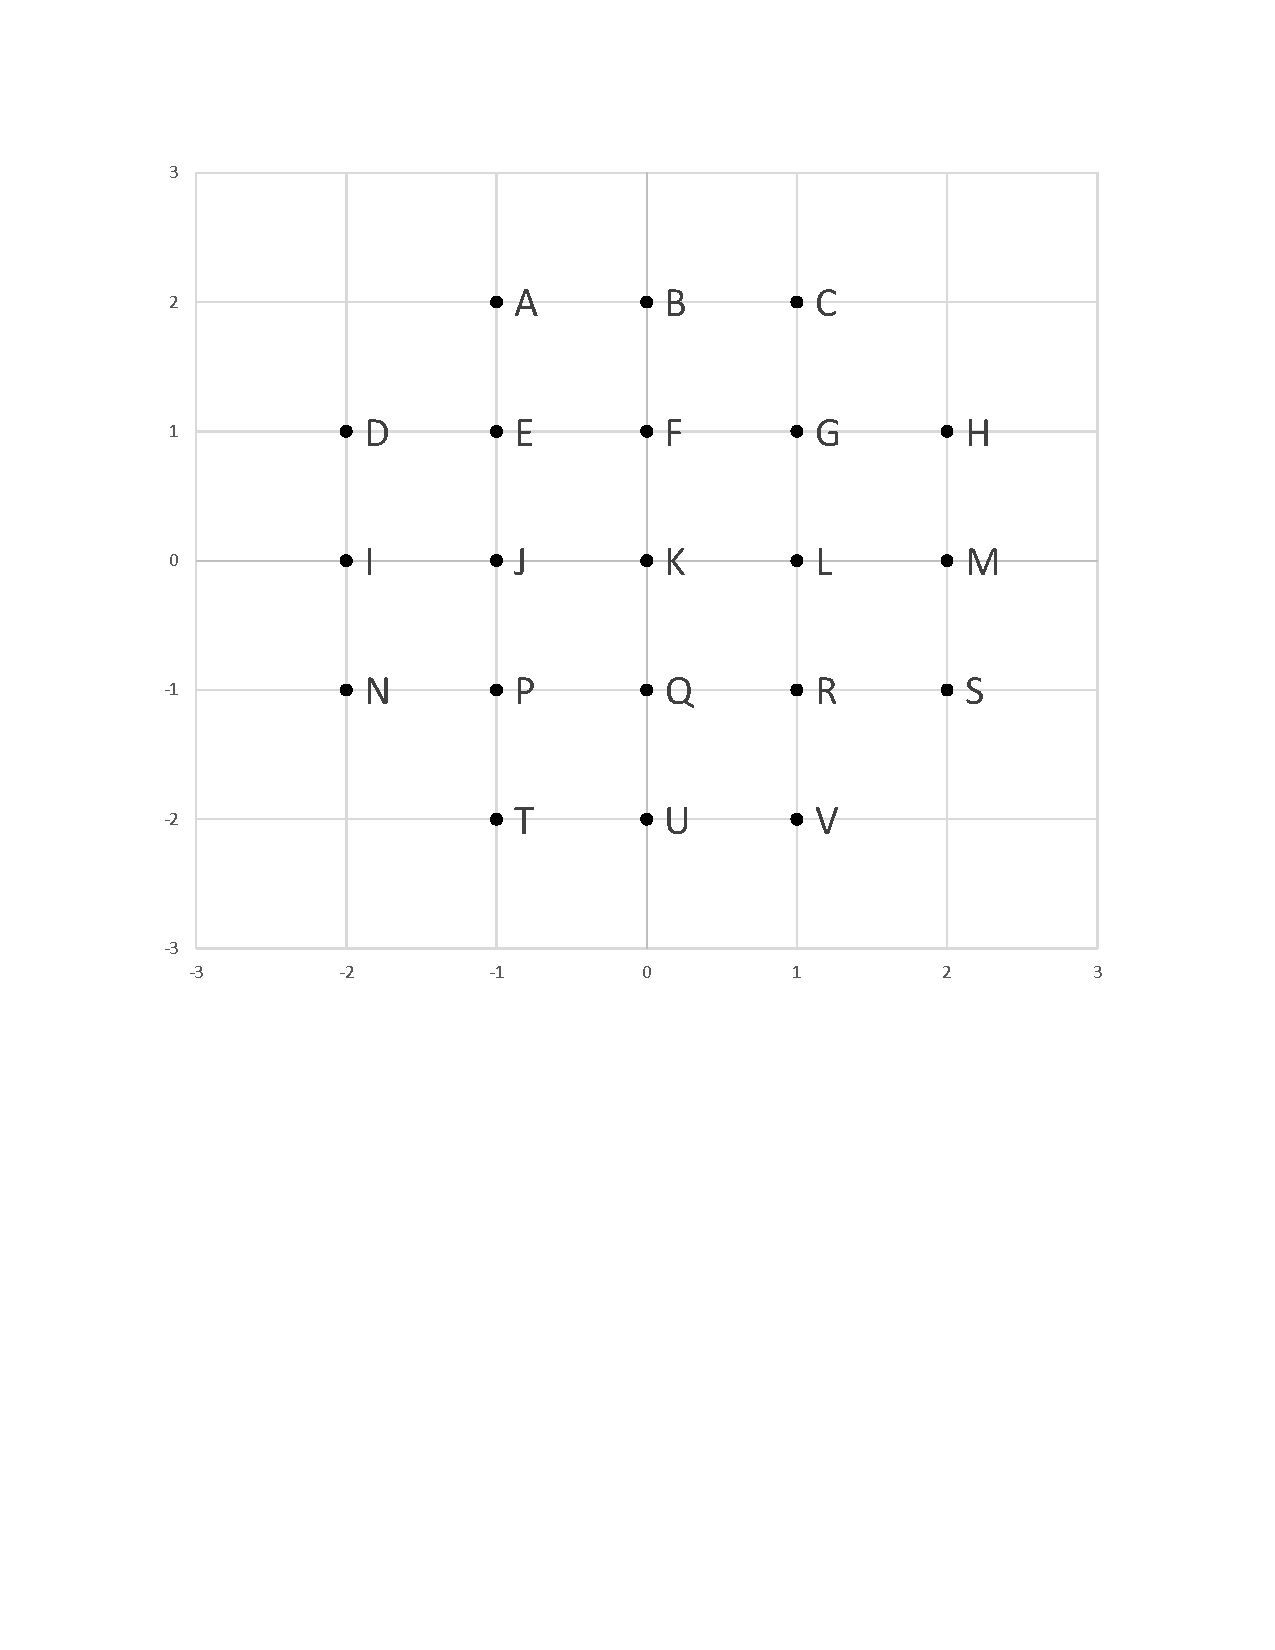
\includegraphics[width=.6\textwidth]{Perturb_Grid_fig.pdf}
			\label{Perturb_Grid_fig}
		\end{figure}

		The constant term is $f(\sf K)$.

		To find the first derivatives we evaluate our function at the points indicated.
		\begin{align}
			f_x(x,y) & = \frac{f(\sf L)-f(\sf J)}{2\ve} \nonumber \\
			f_y(x,y) & = \frac{f(\sf F)-f(\sf Q)}{2\ve} \nonumber
		\end{align}

		Second deriviatives are:
		\begin{align}
			f_{xx}(x,y) & = \frac{\frac{f(\sf L)-f(\sf K)}{\ve} - \frac{f(\sf K)-f(\sf J)}{\ve}}{\ve} = \frac{f(\sf L)-2f(\sf K)+f(\sf J)}{\ve^2} \nonumber \\
			f_{yy}(x,y) & = \frac{\frac{f(\sf F)-f(\sf K)}{\ve} - \frac{f(\sf K)-f(\sf Q)}{\ve}}{\ve} = \frac{f(\sf F)-2f(\sf K)+f(\sf Q)}{\ve^2} \nonumber \\
			f_{yy}(x,y) & = \frac{\frac{f(\sf G)-f(\sf E)}{2\ve} - \frac{f(\sf R)-f(\sf P)}{2\ve}}{2\ve} = \frac{f(\sf G)-f(\sf E)-f(\sf R)+f(\sf P)}{4\ve^2} \nonumber
		\end{align}

		Third deriviatives are:
		\begin{align}
			f_{xxx}(x,y) & = \frac{\frac{f(\sf M)-2f(\sf L)+f(\sf K)}{\ve^2} - \frac{f(\sf K)-2f(\sf J)+f(\sf I)}{\ve^2}}{2\ve} =\frac{f(\sf M)-2f(\sf L)+2f(\sf J)-f(\sf I)}{2\ve^3} \nonumber \\
			f_{xxy}(x,y) & = \frac{\frac{f(\sf H)-f(\sf F)-f(\sf S)+f(\sf Q)}{4\ve^2} - \frac{f(\sf F)-f(\sf D)-f(\sf Q)+f(\sf N)}{4\ve^2}}{2\ve} \nonumber \\
			             & = \frac{f(\sf H)-2f(\sf F)-f(\sf S)+f(\sf D)+2f(\sf Q)-f(\sf N)}{8\ve} \nonumber \\
			f_{xyy}(x,y)& = \frac{\frac{f(\sf A)-f(\sf J)-f(\sf C)+f(\sf L)}{4\ve^2} - \frac{f(\sf J)-f(\sf T)-f(\sf L)+f(\sf V)}{4\ve^2}}{2\ve} \nonumber \\
			             & = \frac{f(\sf A)-2f(\sf J)-f(\sf C)+f(\sf T)+2f(\sf L)-f(\sf V)}{8\ve} \nonumber \\
			f_{yyy}(x,y) & = \frac{\frac{f(\sf B)-2f(\sf F)+f(\sf K)}{\ve^2} - \frac{f(\sf K)-2f(\sf Q)+f(\sf U)}{\ve^2}}{2\ve} =\frac{f(\sf B)-2f(\sf F)+2f(\sf Q)-f(\sf U)}{2\ve^3} \nonumber
		\end{align}



\newpage
%exercises
\section*{Exercises}\label{Perturb_HW} 

	% 1
	\begin{exercise} \label{Perturb_HW_Cubic}
		Following the example in equations \eqref{Perturb_Fxu2derv} and \eqref{Perturb_quad}, find the formula for the cubic term, $x_{uuu}(u_0)$, as a function of the derivatives of the $F$ function and the lower-order derrivatives of the $x$ function, i.e. $x(u_0)$, $x_u(u_0)$ and $x_{uu}(u_0)$.
	\end{exercise}

	% 2
	\begin{exercise} \label{Perturb_HW02_GEApprox}
		Consider the following static general equlibrim model.  Firms have a demand for labor curve given by $n^d = \left[\frac{(1-\alpha)z}{w}\right]^{\tfrac{1}{\alpha}} k$, where $z$ is the level of technology, $w$ is the wage rate, $k$ is a fixed capital stock, and $\alpha$ is a capital share parameter from a Cobb-Douglas production function.  Given this, the profits earned by the firm are $\pi = zk^\alpha (n^d)^{1-\alpha} - w n^d$.  The supply of labor by households is $n^s = h - \frac{b}{w(1+b)}(wh+\pi-t)$, where $h$ is the time endowment of the household, is $t$ is a lump-sum tax, and $b$ is a weight in utility on leisure versus consumption of goods.  Assuming a unit measure of both households and firms, use the following parameter values $\alpha = .33$, $k=5$, $z=1$, $b=2$, $t=.1$ and $h=24$.

		Find the market-clearing wage rate using {\tt fsolve}.  Find a first-order approxmation for wage as a function of $k$.  Approximate about $k=5$.  

		Find a second-order approximation also about $k=5$.

		Set up a grid on the space between $k=1$ and $k=15$. Use {\tt fsolve} to find the equilibrium value of the wage at each point on the grid.

		Plot the grid solution, the linear and quadratic approximations on the same graph.

		Repeat the above exercise when the approximation point is $k=10$.
	\end{exercise}

	% 3
	\begin{exercise} \label{Perturb_HW_Bivar_Grid}
		For the function $F(y,x) =(x^{.35} + .9x - y)^{-2.5} - .95(y^{.35} + .9y )^{-2.5} = 0$, simplify and then use perturbation methods to find the cubic approximation of $y=G(x)$ about the point $x_0=100$.  In this case, $y_0=G(x_0)=49.2166$.

		Write out the functional form of this polynomial with numbers for coefficients.

		Set up a grid on the space between $x=99$ and $x=101$. Use {\tt fsolve} to find the equilibrium value of $y$ at each point on the grid.

		Plot the difference between the linear, quadratic and cubic approximations and the grid solution on the same graph over the range $x\in(99,101)$.
	\end{exercise}

	% 4
	\begin{exercise} \label{Perturb_HW_BM_NoStoch}
		For the \citet{BrockMirman1972} model in section \ref{Perturb_DGE} with the default parameter values find the scalar values of $H_X$ and $H_{XX}$.  Use analytical derivatives.

		Plot the the linear and quadratic approximations to policy function $K' = H(K)$.  Compare this with the closed form solution from the notes.
	\end{exercise}

	% 5
	\begin{exercise} \label{Perturb_HW_BM}
		For the \citet{BrockMirman1972} model with the default parameter values find the scalar values of $H_X$, $H_Z$, $H_{XX}$, $H_{XZ}$, $H_{ZZ}$ and $H_{vv}$.  Use numerical derivatives.

		Plot the three-dimensional surface plot for the policy function $K' = H(K,z)$.  Compare this with the closed form solution from the notes and the two approximations from the DSGE chapter Exercise 8 and the Linearization chapter Exercise 1.
	\end{exercise}

	% 6
	\begin{exercise} \label{Perturb_HW_BAse}
		Repeat Exercise \ref{Perturb_HW_BM} above using the baseline model from section 6 in the linearization chapter.  Generate figures similar to those you generated in the Linearization chapter in Exercise 7.  Compare this plot with the one from that exercise.
	\end{exercise}


\end{spacing}

\newpage

\bibliography{BootCampText}

\end{document}